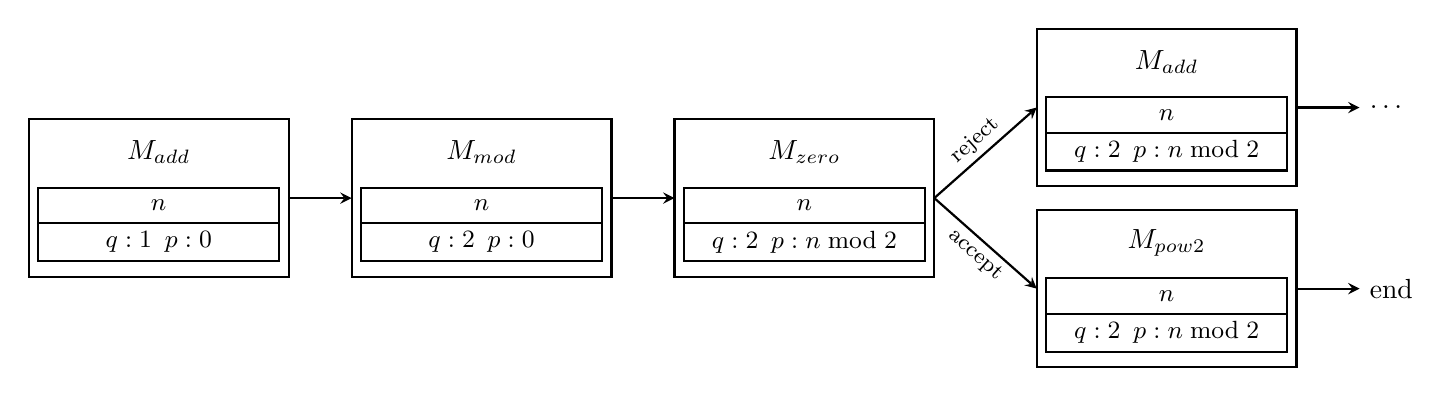
\begin{tikzpicture}[x=1cm, y=1cm, line width=0.8pt,
                    lbl/.style={font=\footnotesize, inner sep=2pt}]
  % ---- layout parameters (cm) ----------------------------------------
  \def\mw{3.3}     % width of one machine box
  \def\mh{2.0}     % height of one machine box
  \def\gap{0.8}    % horizontal gap between machines in the row
  \def\fork{1.3}   % horizontal gap before the stacked pair
  \def\vgap{0.3}   % vertical gap between the two stacked machines

  % #1 = title, #2 = counters
  \tikzset{
    pics/machine/.style 2 args={code={
      % outer box (lower-left corner at the pic's position)
      \draw (0,0) rectangle (\mw,\mh);
      \coordinate (-W) at (0,\mh/2);      % midpoint of left edge
      \coordinate (-E) at (\mw,\mh/2);    % midpoint of right edge
      % title
      \node at (\mw/2,1.58) {#1};
      % stacked boxes: n on top, counters below, sharing one border
      \draw (0.12,0.2) rectangle (\mw-0.12,1.13);
      \draw (0.12,0.68) -- (\mw-0.12,0.68);
      \node at (\mw/2,0.905) {\small $n$};
      \node at (\mw/2,0.44) {\small #2};
    }}
  }
  % row of three machines
  \pic (m1) at (0,0)                {machine={$M_{\text{add}}$}{$q : 1 \enspace p : 0$}};
  \pic (m2) at ({1*(\mw+\gap)},0)   {machine={$M_{\text{mod}}$}{$q : 2 \enspace p : 0$}};
  \pic (m3) at ({2*(\mw+\gap)},0)   {machine={$M_{\text{zero}}$}{$q : 2 \enspace p : n \bmod 2$}};

  % column of two machines, centred vertically on the row
  \pic (m4) at ({3*\mw+2*\gap+\fork},{(\mh+\vgap)/2})   {machine={$M_{\text{add}}$}{$q : 2 \enspace p : n \bmod 2$}};   % top
  \pic (m5) at ({3*\mw+2*\gap+\fork},{-(\mh+\vgap)/2})  {machine={$M_{\text{pow2}}$}{$q : 2 \enspace p : n \bmod 2$}};  % bottom

  \node[anchor=west] (next) at ([xshift=\gap cm]m4-E) {\dots};
  \node[anchor=west] (end) at ([xshift=\gap cm]m5-E) {end};

  % arrows
  \draw[-stealth] (m1-E) -- (m2-W);
  \draw[-stealth] (m2-E) -- (m3-W);
  \draw[-stealth] (m3-E) -- node[lbl, above, sloped] {reject} (m4-W);
  \draw[-stealth] (m3-E) -- node[lbl, below, sloped] {accept} (m5-W);
  \draw[-stealth] (m4-E) -- (next);
  \draw[-stealth] (m5-E) -- (end);
\end{tikzpicture}